%TODO:
% - warum CuSO4?
% - warum ist cp falsch?
% - mehr beispielbilder (ausdrucke) incl. verweisen darauf im text
% - conclusion too short?

\documentclass[a4paper]{scrartcl}

\usepackage[utf8]{inputenc}
\usepackage[english]{babel}
\usepackage{lmodern} 
\usepackage[T1]{fontenc}
\usepackage{booktabs}
\usepackage{multirow}
\usepackage{wrapfig}


% PAKETE
\usepackage{siunitx}
\usepackage{graphicx}
\usepackage[usenames,dvipsnames]{xcolor}
\usepackage{placeins}
\usepackage{longtable}
\usepackage{enumitem}
\usepackage{bbm}

\usepackage{amssymb} % math symbols
\usepackage{amsmath} % ams
\usepackage{amsfonts} % mathmatical fonts

% caption indenting
 \usepackage[format=plain,indention=0em,labelfont=bf,margin=1em]{caption} 
 \usepackage{subfig} %subfigures ^^
\usepackage[protrusion=true,expansion=true]{microtype} % denser font, "-" behind line
\usepackage{esint} % nicer double and triple integrals
\usepackage{fancyhdr} % fancy headers
\usepackage[colorlinks=true,linkcolor=black,citecolor=black,filecolor=black,urlcolor=black]{hyperref}



% EINSTELLUNGEN
\sisetup{seperr,repeatunits=false}
\numberwithin{equation}{section}
\numberwithin{figure}{section}
\numberwithin{table}{section}

% EIGENE FUNKTIONEN
\newcommand{\re}{\operatorname{Re}}
\newcommand{\im}{\operatorname{Im}}
\newcommand{\gquote}[1]{\glqq #1 \grqq}

\newcommand{\eq}[2]{\begin{equation}#1\label{#2}\end{equation}}
\newcommand{\eqand}[0]{\hspace{.25cm} \bigwedge \hspace{.25cm}}
\newcommand{\grafik}[2]{\begin{figure}[h]\centering \includegraphics[width=10cm]{#1.eps}  \caption{#2} \label{#1} \end{figure} }
\newcommand{\grafikq}[3]{\begin{figure}[h]\centering \includegraphics[width=10cm]{#1.eps}  \caption[#2]{#3} \label{#1} \end{figure} }
\newcommand{\tbl}[3]{\begin{table}[h]\caption{#1}\label{#2}\begin{center}#3\end{center}\end{table}}
\newcommand{\Abbildung}[1]{\textsl{Abbildung \ref{#1}}}
\newcommand{\AbbildungI}[1]{\textsl{(Abbildung \ref{#1})}}
\newcommand{\Tabelle}[1]{\textsl{Tabelle \ref{#1}}}
\newcommand{\TabelleI}[1]{\textsl{(Tabelle \ref{#1})}}
\newcommand{\Formel}[1]{(\ref{#1})}
\renewcommand{\d}{\mathrm{d}}
\newcommand{\ve}[1]{\mathbf{ #1} }

\title{Ma 3: Pulsed Nuclear Magnetic Resonance (NMR)}
\subtitle{Tutor: C. Meier}
\author{Benjamin Huber, Carolin Wille}
\date{January 16, 2012}

\begin{document}
\thispagestyle{empty}
\maketitle
\tableofcontents
\clearpage


\section{Introduction}
The Pulsed Nuclear Magnetic Resonance method was developed in 1946. Since then it has greatly influenced medical imaging (NMR tomography) and the analysis of molecules in liquids and solids by allowing certain conclusions about the field near the nucleus with total spin $\ve I \neq 0$.


\subsection{Nuclear Spins in a Static Setting}
In nuclei with an even number of neutrons and protons, the total spin vanishes due to every energy level being occupied by one spin up and one spin down particle. For atoms with either uneven proton or neutron number, this can not be the case. Instead there will be a non-vanishing total nuclear spin leading to a magnetic moment
\eq{\ve \mu_I = \gamma_I \hbar \ve I =g_K \mu_K \ve I,}{}
where $\gamma_I$ is the gyromagnetic relationship, $g_K$ the gyromagnetic g-factor and $\mu_K$ the nuclear magneton. This magneton is defined parallel to the Bohr magneton
\eq{\ve \mu_K = \frac{m_p}{m_e}\ve \mu_B .}{}

When applying an external magnetic field, these magnetic moments will orient parallel to this field. Due to the interaction between dipole and field the energy will shift by
\eq{\Delta E = g_K\mu_K B_0 m_I ,}{}
with $m_I$ being the magnetic quantum number with values $0,\pm 1,\dots,\pm I$.

As for the corresponding electronic systems, the occupation numbers for these different energy levels are given by the Boltzmann distribution
\eq{N_i = N_0 \exp\left( -\frac{E_i}{k_B T} \right) .}{}
This distribution leads to a macroscopic magnetization of
\eq{\ve M_0 = \frac{\eta g_K^2 \mu_K^2 I(I+1)}{3 k_B T} \ve B_0}{}
where $\eta = N_0/V$ is the density of nuclear spins.


\subsection{Nuclear Spins in a Dynamic Setting}
A magnetic dipole (or respectively spin) that is not oriented parallel to the external magnetic field performs a movement according to the equation of motion
\eq{\frac{d}{dt}\ve M = \gamma_I \ve M \times \ve B_0 ,}{eq:M1}
leading to a rotation with the Larmor frequency $\ve \omega_0 = -\gamma_I \ve B_0$. If we chose a coordinate system that is rotating with this same frequency, obviously the dipole is at rest, leading to the simple homogeneous ODE
\eq{\frac{d}{dt}\ve M_{rot} = 0.}{eq:Mrot}
Any additional magnetic field $\ve B_1$ will now be represented by an inhomogeneous term on the right side of the equation
\eq{\frac{d}{dt}\ve M_{rot} = \gamma_I \ve M \times \ve B_1.}{}
Assuming that $\ve B_1$ is rotating with $\omega_0$ as well, it is a stationary vector in the new (rotating) system and we thus end up with the same situation as in (\ref{eq:M1}), leading to a similar precession of $\ve M_{rot}$ around $\ve B_1$ (this time in the rotating frame) with frequency $\ve \omega_1 = -\gamma_I \ve B_1$ \cite{carrington} .


\subsection{Pulsed Nuclear Resonance}
As $\ve M_{rot}$ only changes when there is a field $\ve B_1$ and remains constant otherwise (without any other pertubations), it can be timed to stop at any point of its precession. Assuming an equilibrium state (parallel to $\ve B_0$) at the beginning, this precession covers every angle $\alpha$ between $\ve B_0$ and $\ve M_{rot}$ (respectively $\ve M$, as this angle does not change with (\ref{eq:Mrot}) ). Prominent are the $\alpha = \pi/2$ and $\alpha = \pi$ configurations.

Once the rotating field $\ve B_1$ is turned off, relaxation of the spins back to the equilibrium position can be observed. The timescale of these events as well as the strength of the resulting radiation contains information about the investigated sample.


\subsection{Relaxation}
\label{sec:relax}
In general there needs to be a pertubation of the clean system of (\ref{eq:M1}) for it to allow any relaxation to the equilibrium state at all. In the experiment these are spin-spin and spin-lattice interactions.

\subsubsection*{Spin-Lattice Relaxation}
The spin-lattice interaction is caused by the magnetic moments of the other atoms.\footnote{The nomenclature Spin-\emph{Lattice} Relaxation seems to promote the use for solids even though the Bloch equations turn out to be of limited use for solids and are more precise for liquids.} It causes the relaxation along the direction of $\ve B_0$. The corresponding Bloch equation is
\eq{\frac{dM_z}{dt} = -\frac{M_z - M_0}{T_1}}{eq:B1}
\eq{\Rightarrow  M_z = M_0 \left(1 - 2e^{-t/T_1}\right) .}{}

\subsubsection*{Spin-Spin Relaxation}
Our observed spin is influenced by the magnetic fields created by the other spins surrounding it. This additional field causes a dephasing of the magnetization components perpendicular to $\ve B_0$. In the form of Bloch equations this reads\footnote{Note that the integrations are not strictly true because $M_x$ and $M_y$ refer to the not rotating frame, but it might turn out to be just as good an approximation as the original Bloch equation (\ref{eq:B2}).}
\eq{\frac{dM_{x,y}}{dt} = -\frac{M_{x,y}}{T_2}}{eq:B2}
\eq{\Rightarrow  M_{x,y}=M_0 e^{-t/T_2} .}{}

Not assuming the approximation of independent coordinates leading to the integrals of above, the total differential equation reads
\eq{\frac{d}{dt}\ve M = \gamma_I B_0 \ve M \times \ve e_z - \ve e_x \frac{M_x}{T_2} - \ve e_y \frac{M_y}{T_2} - \ve e_z \frac{M_z - M_0}{T_1} }{eq:Mtotal}
where the coordinate direction $\ve e_z$ was chosen such that $\ve B_0 = B_0 \ve e_z$.

\subsubsection*{Free Induction Decay}
The spin-spin relaxation is caused by the change in amplitude of $\ve B_0$. It is just as well possible though that the external magnetic field itself is not perfectly homogeneous, leading to a similar decay
\eq{M_{x,y} = M_0 e^{-t/T_2^*} .}{}
As the inhomogeneity of the external field must be on a much larger lengthscale and thus effects more magnetizations more strongly than the spin-spin interaction, we can assume $T_2^* \ll T_2$.


\subsection{Methods of Measurement}
\label{sec:methods}
Because the different timescales $T_{1,2}$ and $T_2^*$ are all the result of different processes, it can be interesting to get quantitative values for all the independently.

\subsubsection*{Measurement of $T_2^*$}
$T_2^*$ is the shortest of the three timescales \cite{skript}. It is measured by flipping the spins into the x-y-plane with a $\pi/2$ pulse and observing the relaxation. The final value gives information about the inhomogeneity of the external field ${\Delta B}$. In the case of gaussian distributed inhomogeneities this is
\eq{{\Delta B} = \frac{\ln(2)}{\gamma_I T_2^*} .}{eq:deltaB}

\subsubsection*{Measurement of $T_1$ (Inversion Recovery)}
For this measurement a full $\pi$ pulse is applied. This will flip the spin to the opposite direction. After a while $\tau$ a $\pi/2$ pulse brings the spin back to the x-y-plane where it can be measured similar to the measurement of $T_2^*$. The dependence of the initial amplitude after the $\pi/2$ pulse on the time $\tau$ gives the constant $T_1$.

\subsubsection*{Measurement of $T_2$ (Spin Echo)}
The decrease in intensity is caused by dephasing due to different precession rates caused by different magnet fields. The idea of the Spin Echo method is to get rid of the (assumed to be constant) inhomogeneity of the external field. This is achieved by applying a $\pi$ pulse after some time $\tau$. The initially dephasing magnetizations will now rephase because their relative velocities only depend on the magnetic field and thus did not change when the $\pi$ pulse was applied. The only remaining term is the spin-spin interaction that was changed with the pulse and thus causes further dephasing over the whole measurement. Several $\frac{\pi}{2},\tau,\pi,\tau,$echo sequences with varying $\tau$ will thus reveal the constant $T_2$.

\subsubsection*{Carr-Purcell-Method}
To decrease the time needed for the measurements of $T_2$ Carr and Purcell \cite{purcell} introduced a method to take several measurements in one run consisting of the pulses $\frac{\pi}{2},\tau,\pi,\tau,\pi,...\,$. While this reduces the error due to diffusion in the sample the error of the $\pi$ pulse accumulates over time.

\subsubsection*{Meiboom-Gill-Method}
Meiboom and Gill fixed this accumulation by alternating the direction of the pulses such that an inaccuracy $\delta$ for the $\pi$ pulse vanishes $(\pi+\delta)-(\pi+\delta)=0$. Thus every second measurement is not influences by this error with a sequence of $\frac{\pi}{2},\tau,\pi,\tau,-\pi,\tau,\pi,...\,$.

\clearpage
\section{Experiment}
\subsection{Tuning of resonance frequency}
First, the LC-circuit and the frequency synthesizer were tuned to resonance frequency. The expected value of the Larmor frequency $f_0=\frac{\omega_0}{2\pi}=\frac{\gamma_\text{proton}}{2\pi} B_0 =  \SI{21.287}{MHz}$, where $\gamma_\text{proton}=2.675*10^8/(\text{s}*\text{T})$ and $B_0\simeq\SI{0.50(2)}{T}$ \cite{hersteller} is close to the frequency $f=\SI{21.029}{MHz}$, which resulted in the highest FID signal. The LC-circuit was adjusted via the capacity of a capacitor to match also the resonance frequency again via optimizing the FID signal.
\subsection{Determination of pulse duration}
The length of a pulse determines the rotation angle. For the $\pi/2$ pulse, a maximal FID signal indicates the correct length . For the $\pi$ pulse, different methods were used to adjust its length. A first estimate can be gained also by the FID signal, which should be minimal after a single $\pi$ pulse. Another method was to compare Meiboom-Gill- and Carr-Purcell-Series, which should be most similar for minimal error of the $\pi$ pulse. However, both methods lead to different optimal $\pi$ pulse lengths. As the results for the CP series were not optimal for any $\pi$ pulse length, the length was finally determined via the minimal FID signal. Final values: $T\left(\pi/2\right) = 3.06\,\text{ms}$ and $T\left(\pi\right) = 6.00\,\text{ms}$. 


\section{Analysis}
The aim was to determine the time constants for the Bloch equations describing the behavior of net magnetizations in magnetic fields. To achieve this, the methods described in section \ref{sec:methods} were used on four different samples including mineral oil and CuSO$_4$ in three different concentrations.

\subsection{Free Induction Decay}
As the free induction decay only depends on the external field, it is not expected to change with a change of samples. To confirm this expectation, two samples were investigated with different (deliberate) inhomogeneities in the external field induced by additional field gradients $B_x, B_y, B_z, B_{zz}$. Two plots of the free induction decay with different amount of inhomogeneities can be found in appendix A. The optimal settings for the external fields\footnote{Inhomogeneity balancing function of $B_y=2.1*7.1 \mu \text{T} /\text{mm} = 14.91 \frac{\mu \text{T}}{\text{mm}} $ and $B_{zz} = -1.9 * 20 \mu \text{T} / \text{mm}^2 =-38 \frac{\mu \text{T}}{\text{mm}^2} $. Scaling factors obtained from \cite{hersteller}.} were applied to a sample of mineral oil and of CuSO$_4$ (see figure \ref{fig:fid}). Both resulted in identical values for $T_2^* = (0.441\pm 0.015)\,\text{ms}$ (weighted mean).

With the relation between $T_2^*$ and the inhomogeneity of the magnetic field $\Delta B$ from equation (\ref{eq:deltaB}) and the gyromagnetic moment of the proton $\gamma=2.68\cdot 10^8 \, \text{s}^{-1}\text{T}^{-1}$ one gets $\Delta B = (5.86\pm 0.19)\,\mu\text{T}$. As the external field had a strength of about $0.5\,\text{T}$ this corresponds to only $\Delta B / B \approx 10^{-5}$. While one might be able to get another factor of 10 in this relation with very good equipment one clearly can not hope to have a magnetic field homogeneously enough to ignore the influence of $T_2^*$.

\begin{figure}
\centering
	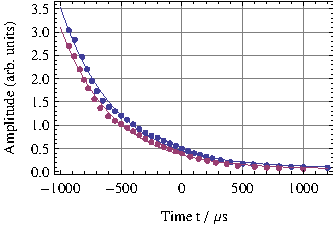
\includegraphics[width=0.5\linewidth]{img/t2st.pdf}
	\caption{\small Intensity over time (with arbitrary 0) of the free induction decay. The mineral oil measurement in blue, the one with a 0.02M CuSO$_4$ solution in magenta. Time constants of the fitted exponential functions with constant noise background are $T_2^*(\text{oil})=(0.448\pm 0.028)\,\text{ms}$, $T_2^*(\text{CuSO}_4)=(0.434\pm 0.030)\,\text{ms}$. }
	\label{fig:fid}
\end{figure}

\subsection{Inversion Recovery}
The measurement of $T_1$ was a straight-forward realization of the inversion recovery method. The three available concentrations of CuSO$_4$ resulted in clearly distinct values for $T_1$. This can be seen with the bare eye in the three different evolutions (see figure \ref{fig:plots}a). For this please note, that the intensity is proportional to the absolute value of the magnetization. With a negative starting magnetization this leads to a sharp bend in the plots.

The fitted time constants are $T_1(0.05)=(20.47\pm 0.61)\,\text{ms}$, $T_1(0.1)=(9.64\pm 0.25)\,\text{ms}$, $T_1(0.2)=(4.25\pm 0.11)\,\text{ms}$.

\subsection{Spin Echo and Meiboom-Gill}
Both, the spin echo and the Meiboom-Gill method to measure $T_2$ resulted in very similar curves, that could have been fitted together were it not for a small difference in intensity (see figures \ref{fig:plots}b and \ref{fig:plots}d). The agreement is significant nonetheless and confirms both the validity of the Meiboom-Gill method as well as that there is only a negligible amount of diffusion in our system.

The fitted time constants for the spin echo methods are $T_2(0.05)=(22.0\pm 1.2)\,\text{ms}$, $T_2(0.1)=(9.85\pm 0.47)\,\text{ms}$, $T_2(0.2)=(4.42\pm 0.14)\,\text{ms}$ and for the Meiboom-Gill method $T_2(0.05)=(20.17\pm 0.27)\,\text{ms}$, $T_2(0.1)=(10.17\pm 0.43)\,\text{ms}$, $T_2(0.2)=(4.50\pm 0.20)\,\text{ms}$.

\subsection{Concentration Dependence}
The $T_1$ value from the inversion recovery and the $T_2$ values from the spin echo and Meiboom-Gill methods show the same dependence on the concentration of CuSO$_4$ molecules. Considering that $T\rightarrow\infty$ as $c(\text{CuSO}_4)\rightarrow 0$ and that the dependence should be a strictly positive and monotonically decreasing function, a functional relation of the form $T=\frac{a}{c(\text{CuSO}_4)}$ seems most probable. This functional dependence is additionally encouraged by the suggested mechanism of relaxation enhancement: The unpaired electrons of the Cu2+, SO$_4$2- ions exert strong dipole moments and fluctuating magnetic fields, which induce magnetic relaxation of the protons, which encounter those fields. It is thus reasonable, that the decay rate $\Gamma \propto 1/T$ is directly proportional to the probability of a proton to cross the proximity of an ion, which itself is proportional to the ion concentration yielding $1/T \propto c$. 

The corresponding fits can be found in figure \ref{fig:plots}e,f,h. The constant $a$ for the data from the inversion recovery was fit to $a(T_1)=(1.00\pm 0.13)\,\text{msM}$ and for the $T_2$ data to $a(T_2)=(1.023\pm 0.053)\,\text{msM}$ suggesting that for dilute aqueous solution of CuSO$_4$ $T_1\backsimeq T_2$.

\begin{figure} [p]
 \centering
 \begin{tabular}{c c c c}
\multicolumn{2}{c}{
\subfloat[][inversion recovery]
         {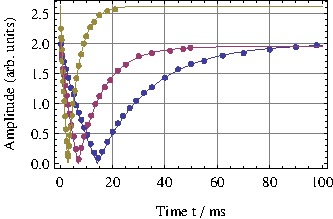
\includegraphics[width=0.49\linewidth]{img/t1.pdf}}
} &
\multicolumn{2}{c}{
\subfloat[][spin echo]
         {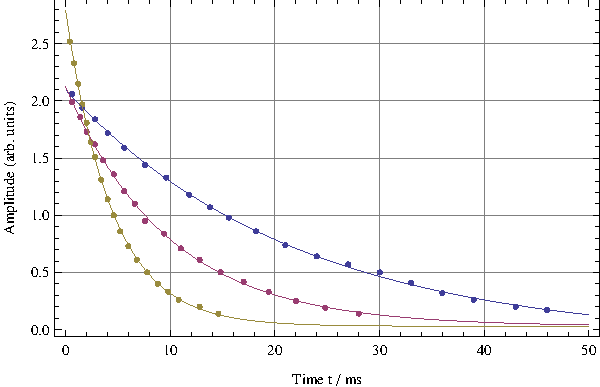
\includegraphics[width=0.49\linewidth]{img/t2se.pdf}}
} \\
\multicolumn{2}{c}{
\subfloat[][Carr-Purcell]
         {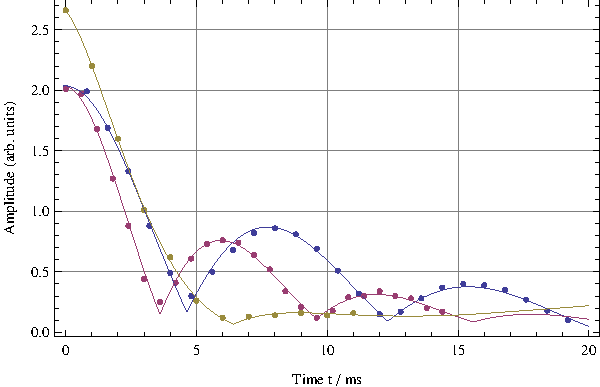
\includegraphics[width=0.49\linewidth]{img/t2cp.pdf}}
} &
\multicolumn{2}{c}{
\subfloat[][Meiboom-Gill]
         {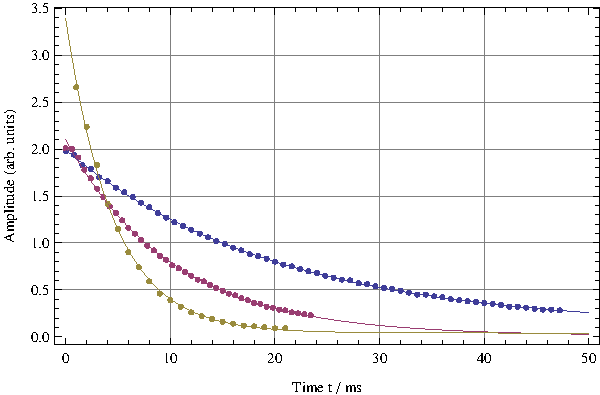
\includegraphics[width=0.49\linewidth]{img/t2mg.pdf}}
} \\
\subfloat[][$T_1$ (inversion)]
         {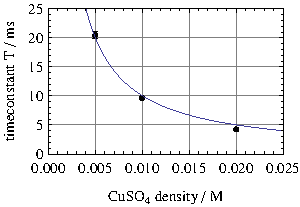
\includegraphics[width=0.23\linewidth]{img/densityt1.pdf}}
&
\subfloat[][$T_2$ (spin echo)]
         {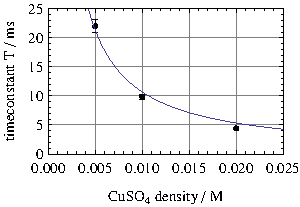
\includegraphics[width=0.23\linewidth]{img/densityt2se.pdf}}
&
\subfloat[][$T_2$ (C-P)]
         {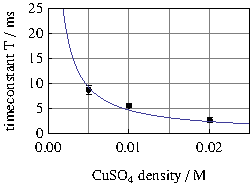
\includegraphics[width=0.23\linewidth]{img/densityt2cp.pdf}}
&
\subfloat[][$T_2$ (M-G)]
         {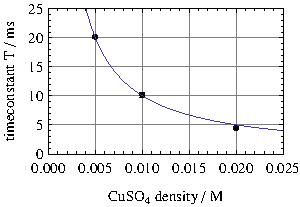
\includegraphics[width=0.23\linewidth]{img/densityt2mg.pdf}}

 \end{tabular}
\caption{
\small \textbf{(a)-(d)} Plots of all four measurement methods for all three concentrations of CuSO$_4$ ($c=0.05$ blue, $c=0.1$ magenta, $c=0.2$ beige). All curves were fitted with a constant noise background (not shown). 
\textbf{(a),(e)} Peak hight in dependence of the time $t$ between $\pi$ and $\pi/2$ pulses of the inversion recovery method.  Corresponding time constants plotted in (e). 
\textbf{(b),(f)} Peak hight in dependence of the time $t$ between $\pi/2$ pulse and echo ($2\tau$) of the spin echo method. Time constants in (f). 
\textbf{(c),(g)} Peak hight in dependence of the time $t$ between first and measured peak (spaced at $2\tau$) for the Carr-Purcell method. See running text for details on the fitted model. Time constants in (g). 
\textbf{(d),(h)} Peak hight in dependence of the time $t$ between first and measured peak (spaced at $2\tau$) for the Meiboom-Gill method. Time constants in (h). 
 }
	\label{fig:plots}
\end{figure}

\subsection{Carr-Purcell}
For the Carr-Purcell method the error of the $\pi$ pulse (and less significantly the $\pi/2$ pulse) have to be considered. A noticeable error will result in an oscillating behaviour as it can be seen in the collected data (cf. figure \ref{fig:plots}c). To account for this oscillation, a more complex model was fitted to the data than anticipated in section \ref{sec:relax}. The (assumed to be constant) error of the $\pi$ pulse causes a constant rotation from the component in the x-y-plane (for the sake of simplicity called the x-component from now on) to the z component and back. The x and z components dephase with the corresponding time constants $T_1$ and $T_2$ leading to the differential equation:
\eq{\frac{d}{dt}x(t) = -\frac{x(t)}{T_2} + \omega z(t)}{}
\eq{\frac{d}{dt}z(t) = -\frac{z(t)}{T_1} - \omega x(t) .}{}
The solution to these ODEs was fitted to the data resulting in not just information for $T_1$ and $T_2$ but also for the error of the pulses ($\omega$ for the $\pi$ pulse and from the initial conditions for the $\pi/2$ pulse).

Unfortunately the solution to these ODEs is ambiguous for $T_1$ and $T_2$ and only the product $T_1 \cdot T_2$ can be fitted from the data. To get realistic values anyway the previous observation that $T_1 \approx T_2$ was included in the fit\footnote{For $T_1=T_2=T$ the solution simplifies to $e^{-t/T} \text{Abs}[x_0 \cos(\omega t)+y_0 \sin(\omega t)]$}. The resulting time constants of $T_{1,2}(0.05)=(8.68\pm0.87)\,\text{ms}$, $T_{1,2}(0.1)=(5.51\pm 0.46)\,\text{ms}$, $T_{1,2}(0.2)=(2.54\pm 0.51)\,\text{ms}$ are too small by a factor of about 2 which is also reflected in the concentration dependence which is for this data $a(\text{Carr-Purcell})=(0.46\pm 0.15)\,\text{msM}$ (see figure \ref{fig:plots}g).% WHY?!?!

The remaining variables that were fitted are useful nonetheless. The error of the $\pi/2$ pulse $\delta(\pi/2) = (23 \pm 18)^\circ$ is rather insignificant for these functions at these values and has thus a large confidence interval that almost includes $\delta = 0$. The pulse length was thus chosen very well even retrospectively. The error of the $\pi$ pulse is more significant $\delta(\pi)=(18.64\pm 0.17)^\circ$. While the value of maximum likelihood is similar as $\delta(\pi/2)$, the much smaller confidence interval suggests, that it would have been possible to find a better pulse length (for example by fitting these Carr-Purcell curves until $\delta(\pi)$ is identical to 0). 


\subsection{Comparisons}
A comparison with other groups that performed the same experiments shows that the Carr-Purcell method resulted consistently in too small values for $T_1$ and $T_2$ (see table \ref{tab:compare}). The other methods resulted in identical or at least compatible values across groups. Where the results deviate too far from the results of the other two groups in this comparison, a confusion about $\tau$ versus $2\tau$ might have been the reason.

\begin{table}[!tbh]
\centering
\small
\begin{tabular}{cccccc}
\toprule
method & constant & our result & group M9 & group M3 (SS11) \\
\midrule 
\midrule
FID & $T_2^* / \text{ms}$ & $0.441\pm 0.015$ & \textcolor{Gray}{$2.5\pm 0.2$} & $0.491\pm 0.018$ \\
& $\Delta B / \mu\text{T}$ & $5.86\pm 0.19$ & $5.4\pm 0.3$ & $5.28\pm 0.18$ \\
\midrule
inversion recovery & $T_1(0.05\,M) / \text{ms}$ & $20.47\pm 0.61$ & $20.7\pm 0.2$ & $23.89\pm0.18$ \\
& $T_1(0.1\,M) / \text{ms}$ & $9.64\pm 0.25$ & $10.3\pm 0.1$ & $12.61\pm0.17$ \\
& $T_1(0.2\,M) / \text{ms}$ & $4.25\pm 0.11$ & $4.5\pm 0.1$ & \textcolor{Gray}{$2.913\pm0.098$} \\
\midrule
spin echo & $T_2(0.05\,M) / \text{ms}$ & $22.0\pm 1.2$ & $19.0\pm 0.7$ & \textcolor{Gray}{$7.76\pm 0.40$} \\
& $T_2(0.1\,M) / \text{ms}$ & $9.85\pm 0.47$ & $10.0\pm 0.1$ & \textcolor{Gray}{$5.267\pm 0.039$} \\
& $T_2(0.2\,M) / \text{ms}$ & $4.42\pm 0.14$ & $4.1\pm 0.1$ & \textcolor{Gray}{$2.367\pm0.037$} \\
\midrule
Meiboom-Gill & $T_2(0.05\,M) / \text{ms}$ & $20.17\pm 0.27$ & \textcolor{Gray}{$13.8\pm 0.6$} & $21.304\,\pm\,$\textcolor{Gray}{$0.047$} \\
& $T_2(0.1\,M) / \text{ms}$ & $10.17\pm 0.43$ & \textcolor{Gray}{$6.4\pm 0.3$} & $11.013\,\pm\,$\textcolor{Gray}{$0.041$} \\
& $T_2(0.2\,M) / \text{ms}$ & $4.50\pm 0.20$ & \textcolor{Gray}{$3.5\pm 0.1$} & $4.287\,\pm\,$\textcolor{Gray}{$0.023$} \\
\midrule
Carr-Purcell$^*$ & $T_{1,2}(0.05\,M) / \text{ms}$ & $8.68\pm0.87$ & $10.1\pm 0.7$ & $5.33\,\pm\,$\textcolor{Gray}{$0.18$} \\
& $T_{1,2}(0.1\,M) / \text{ms}$ & $5.51\pm 0.46$ & $5.1\pm 0.3$ & $4.07\,\pm\,$\textcolor{Gray}{$0.19$} \\
& $T_{1,2}(0.2\,M) / \text{ms}$ & $2.54\pm 0.51$ & $4.3\pm 0.3$ & $2.72\,\pm\,$\textcolor{Gray}{$0.16$} \\
& $\delta(\pi/2) / ^\circ$ & $23 \pm 18$ & & \\
& $\delta(\pi) / ^\circ$ & $18.64\pm 0.17$ & $12\pm 1$ & \\
\midrule
\bottomrule
\end{tabular}
\caption{\small Comparison of experimental results with those of two other groups that worked with the same equipment. Questionable values in gray. \textbf{(*)} While the other groups claimed to get $T_2$ from the Carr-Purcell method they fitted the same function to the data, indicating that they just did not realize that this fit implies $T_1=T_2$. }
\label{tab:compare}
\end{table}


\section{Conclusion}
In this experiment the nuclear magnetic resonance was investigated. Different samples of diluted CuSO$_4$ solutions resulted in different time constants for the Bloch equations consistently implying $T_2^* << T_2 = T_1$ with $T_2^*=(0.441\pm 0.015)\,\text{ms}$ and $T_1=T_2= \frac{(1.02\pm 0.04)\,\text{msM}}{c(\text{CuSO}_4)}$ (for a more detailed listing of all results see table \ref{tab:compare}).

The measurements with the Carr-Purcell method were the only ones, that did not fit this result. The approximations gotten from this for the error in the pulses seem credible, but all time constants are too small by a factor of about 2. While we were not able to find a reason for this, it is consistent with the results of other groups indicating a systematic error or problem with the apparatus being used.


\FloatBarrier
\clearpage
 \bibliographystyle{unsrt}
\bibliography{bib}


\clearpage
\appendix
\section{FID for different Inhomogeneities}
\section{Examples for Carr Purcell and Meiboom Gill Series}

\end{document}


